%\documentclass[poster, a1, landscape, plainboxedsections]{sciposter}
\documentclass[poster, a1, plainboxedsections]{sciposter}

\usepackage{multicol}
\usepackage{amsmath}
\usepackage{amsfonts}
\usepackage{graphicx}
\usepackage{booktabs}
\usepackage{tikz}
\usepackage{pgfplots}
\usepackage{pgfplotstable} % For importing data from a csv

% Allows us to exclude some bars from certain plots, to allow multicoloured plots
\pgfplotsset{
    discard if/.style 2 args={
        x filter/.code={
            \edef\tempa{\thisrow{#1}}
            \edef\tempb{#2}
            \ifx\tempa\tempb
                \def\pgfmathresult{inf}
            \fi
        }
    },
    discard if not/.style 2 args={
        x filter/.code={
            \edef\tempa{\thisrow{#1}}
            \edef\tempb{#2}
            \ifx\tempa\tempb
            \else
                \def\pgfmathresult{inf}
            \fi
        }
    }
}

%\leftlogo[1.1]{McMaster_BlackLogo.pdf}
\leftlogo[1.1]{eng_logo.png}
\rightlogo[1.1]{STaBLLogoWS.png}
\title{A Software Engineering Capstone Infrastructure that Encourages Spreading
Work Over Time and Team}
\author{Spencer Smith, Christopher Schankula, Lucas Dutton and Christopher Anand}
\institute{Computing and Software Department, McMaster University}
\email{smiths@mcmaster.ca}

\begin{document}

\conference{{\bf CSEE\&T 2025}, IEEE Conference on Software Engineering
Education and Training, Apr 28--29, Ottawa, ON, Canada}

\maketitle

\setlength{\columnseprule}{0pt}
\begin{multicols}{2}

\PARstart {H}{ow} can instructors spread out the work in computing capstone
courses across time and among team members? We propose using a GitHub template
that contains all the initial infrastructure, including the folder structure,
text-based template documents and template issues. In addition, we propose each
team begins the year by identifying specific quantifiable individual
productivity metrics for monitoring, such as the count of meetings attended,
issues closed and number of commits. To measure the effectiveness of our
intervention on the distribution of work, we introduce a new fairness metric.

\section{Proposed Process and Infrastructure} \label{SecPropInfrastruc}

\begin{figure}[!h]
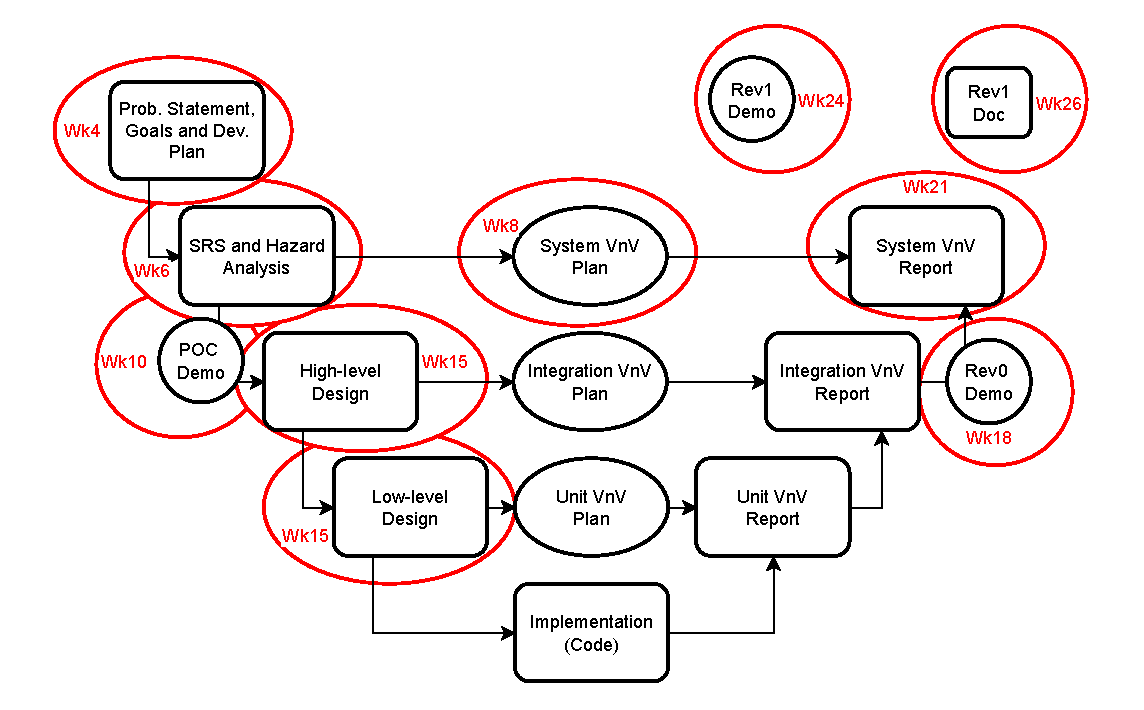
\includegraphics[width=1.0\linewidth]{../figures/CourseStructure.drawio.pdf}
\caption{\label{Fig_VModel} V Model Used for Capstone Deliverables}
\label{FigStructure}
\end{figure}

In an 8-month capstone course, teams of 4--5 follow a V-model process. They
propose a team charter that includes specific quantifiable expectations and
consequences. Team member productivity is reported to the instructor. A template
Github repository is used for standardization and to save time.  

\begin{tikzpicture}[remember picture,overlay]
\node [xshift=-4.5cm,yshift=-3.5cm] at (current page.center)
{

\includegraphics[width=0.1\linewidth]{../figures/captemplate.png}
};
\end{tikzpicture}

\section{Time Spread Before and After Templates}

\begin{figure}[h!]
\centering
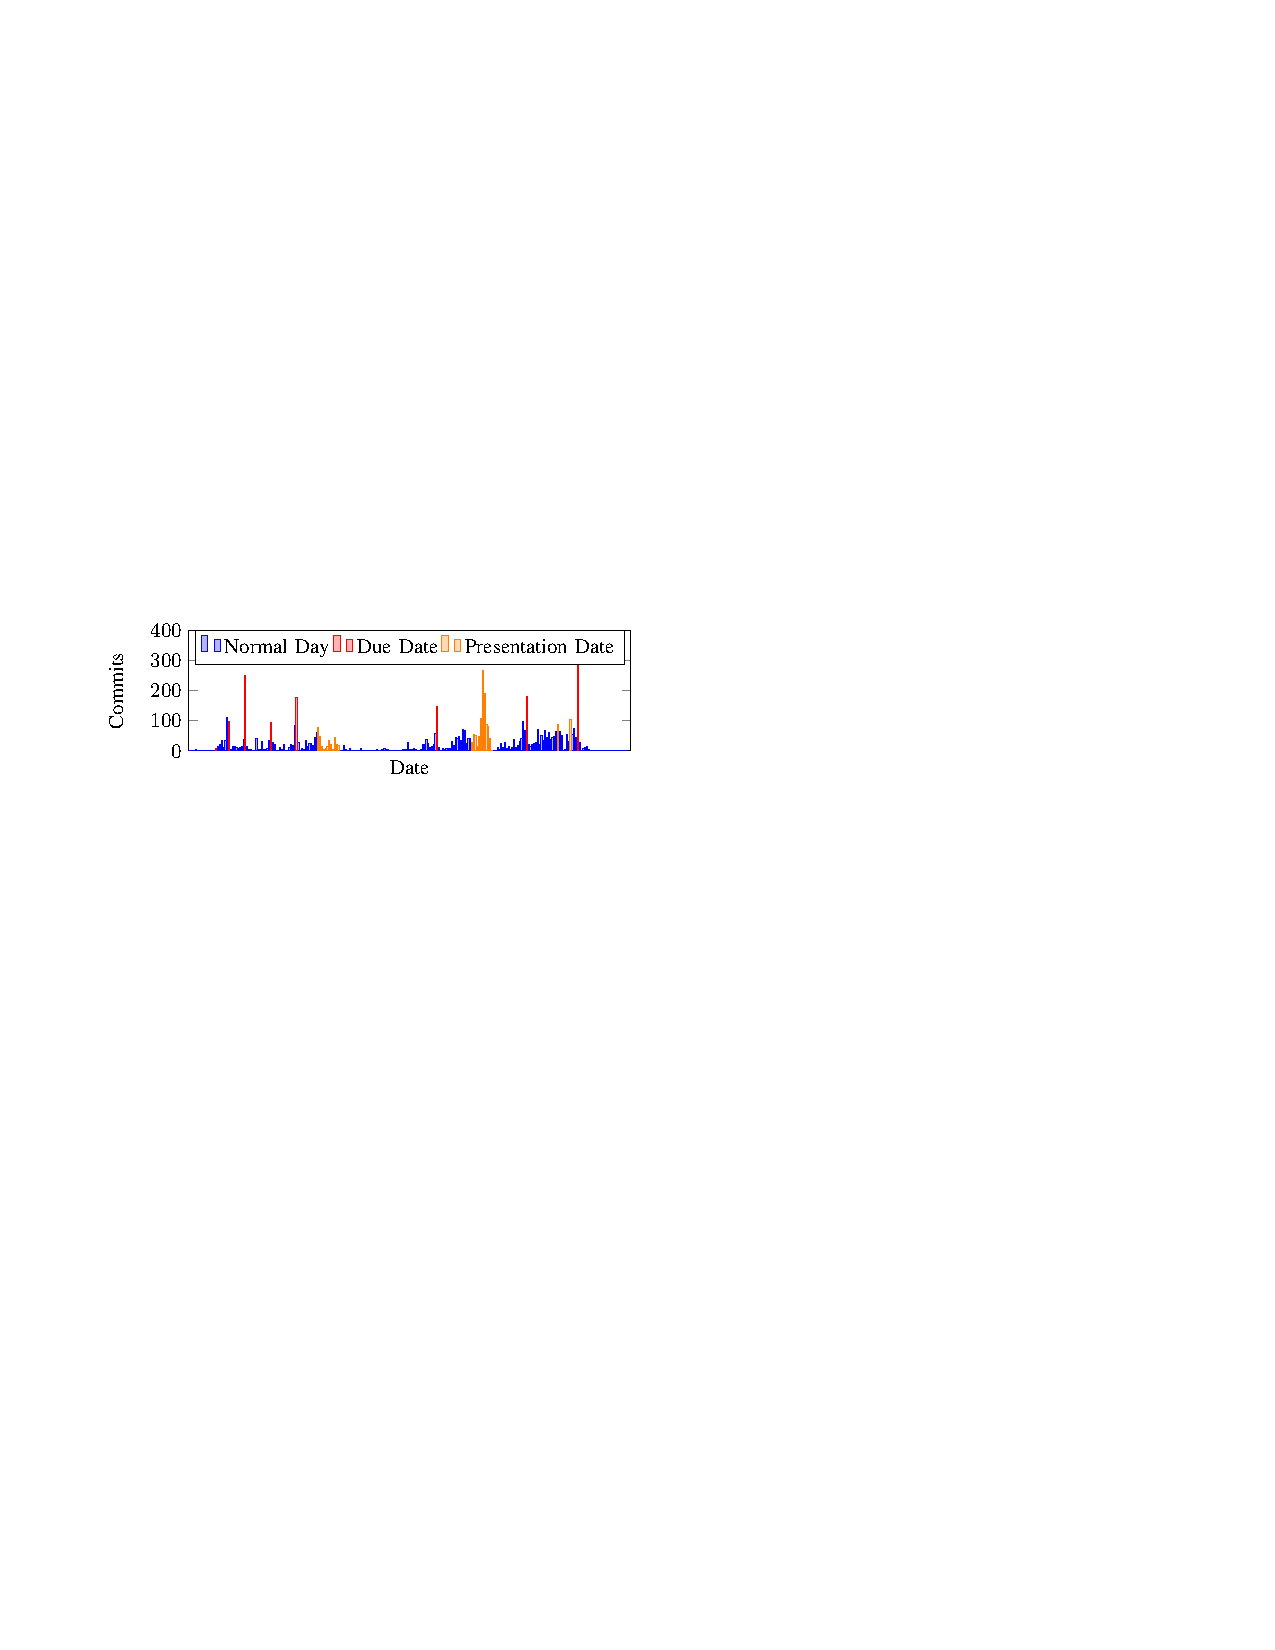
\includegraphics[width=0.9\linewidth]{../figures/HistCommits2022-23.pdf}
\caption{Commits for 2022--2023.}\label{Fig_22_23Timeline}
\end{figure}

\begin{figure}[h!]
\centering
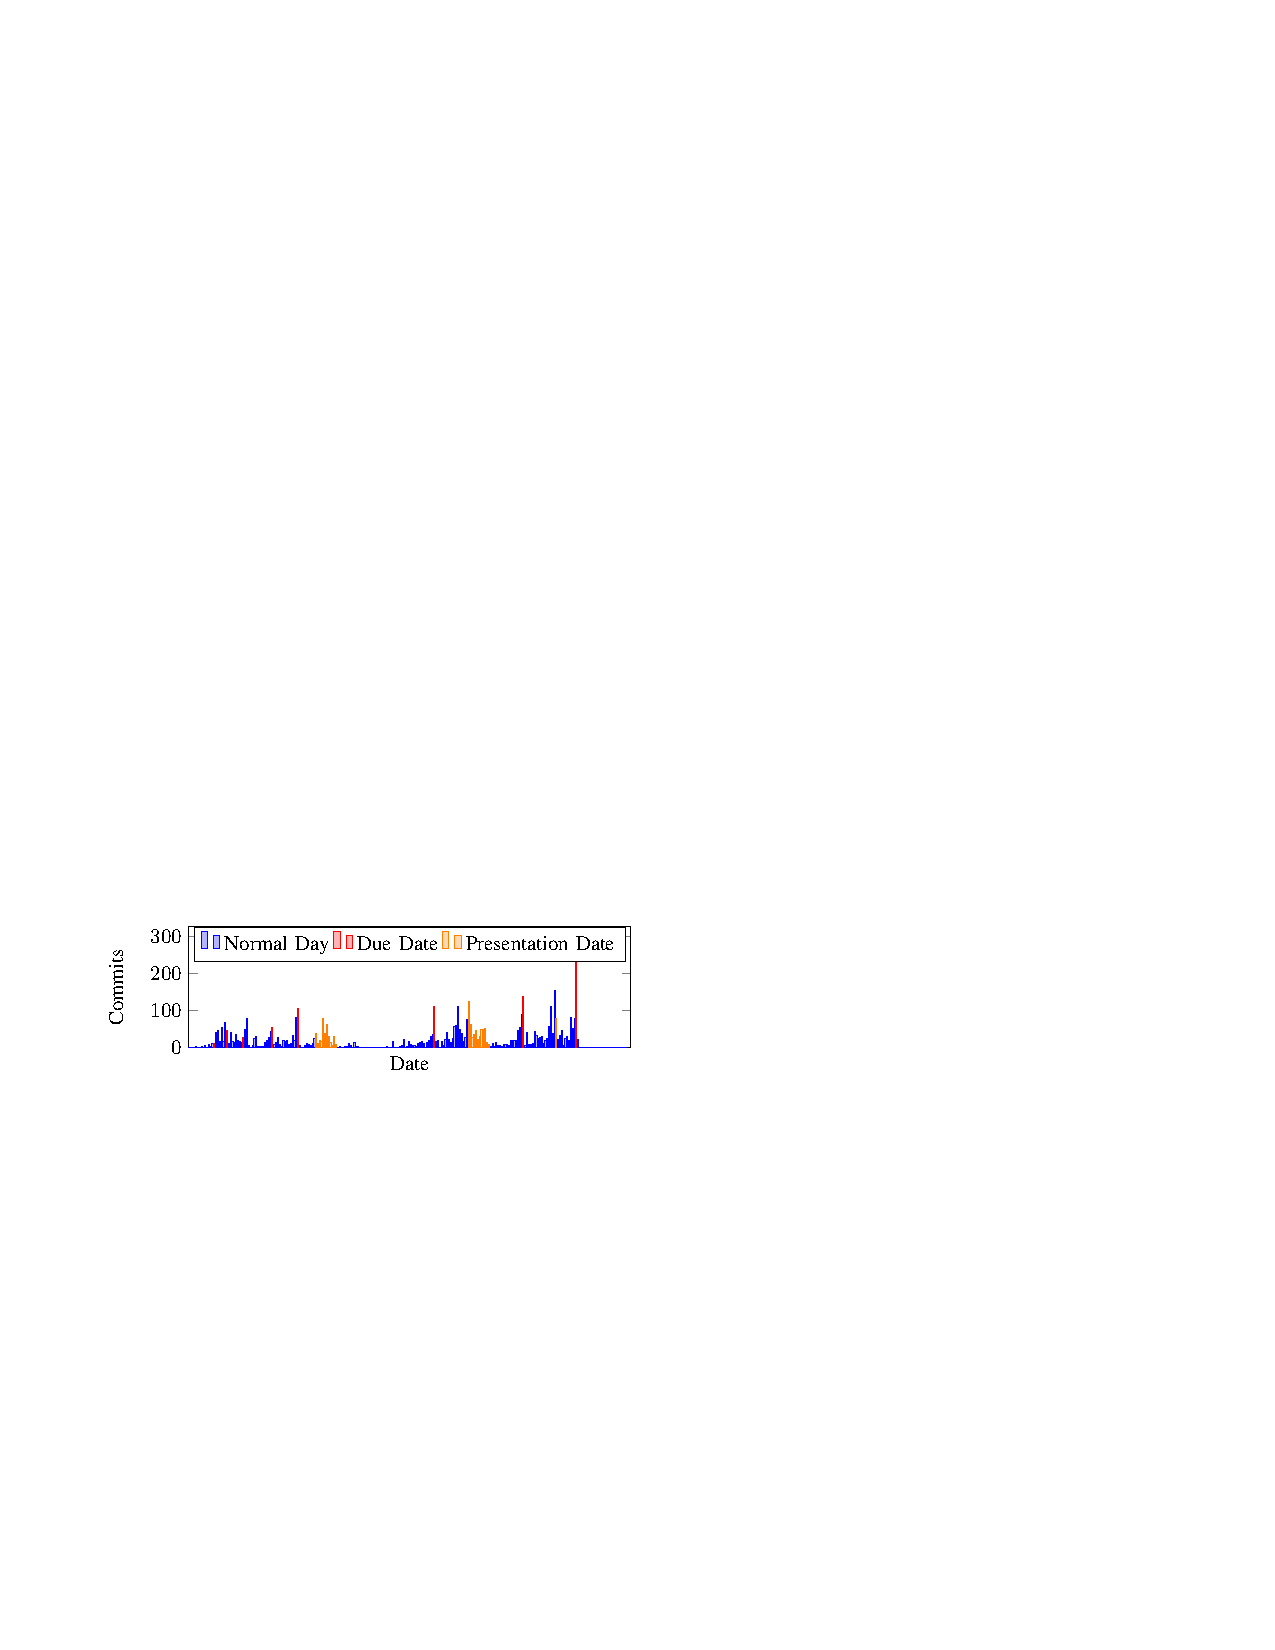
\includegraphics[width=0.9\linewidth]{../figures/HistCommits2023-24.pdf}
\caption{Commits for 2023--2024.}\label{Fig_23_24Timeline}
\end{figure}

The data shows the benefit of partial implementation of the proposed
intervention, but there is still room for improvement. Full elimination of
the deadline effect is unlikely because of the nature of due dates in students' busy
schedules.

\begin{table}
\caption{T0 on deadline, T2 up to two days prior}
\centering
\begin{tabular}{@{}lrrr@{}}
\toprule
\textbf{Metric} & \textbf{2022/23 Value} & \textbf{2023/24 Value} \\ 
\midrule
Total Commits & 6140 & 5120 \\
T0 Commits & 1471 (23.96\%) & 942 (18.40\%) \\
T2 Commits & 2377 (38.71\%) & 1872 (36.56\%) \\ 
\bottomrule
\end{tabular}
\end{table}

\section*{Team Fairness Before and After Templates}

$$
\text{fairness}(C) = 1 - \frac{ \sum\limits_{c, x \in C, c > x} (c-x)}{(\left|C\right| -
1) \cdot \sum\limits_{c \in C} c}
$$

\noindent where $C$ is the multiset of teammates' numbers of commits to the 
repository.

The index computes one minus the sum of the difference between each teammate's
commits and those who committed less than them, normalized by the number of
teammates (excluding themselves) and the total number of commits. This yields a
value from 1 to 0, called the \textit{fairness} index.

\begin{figure}[h]
\centering
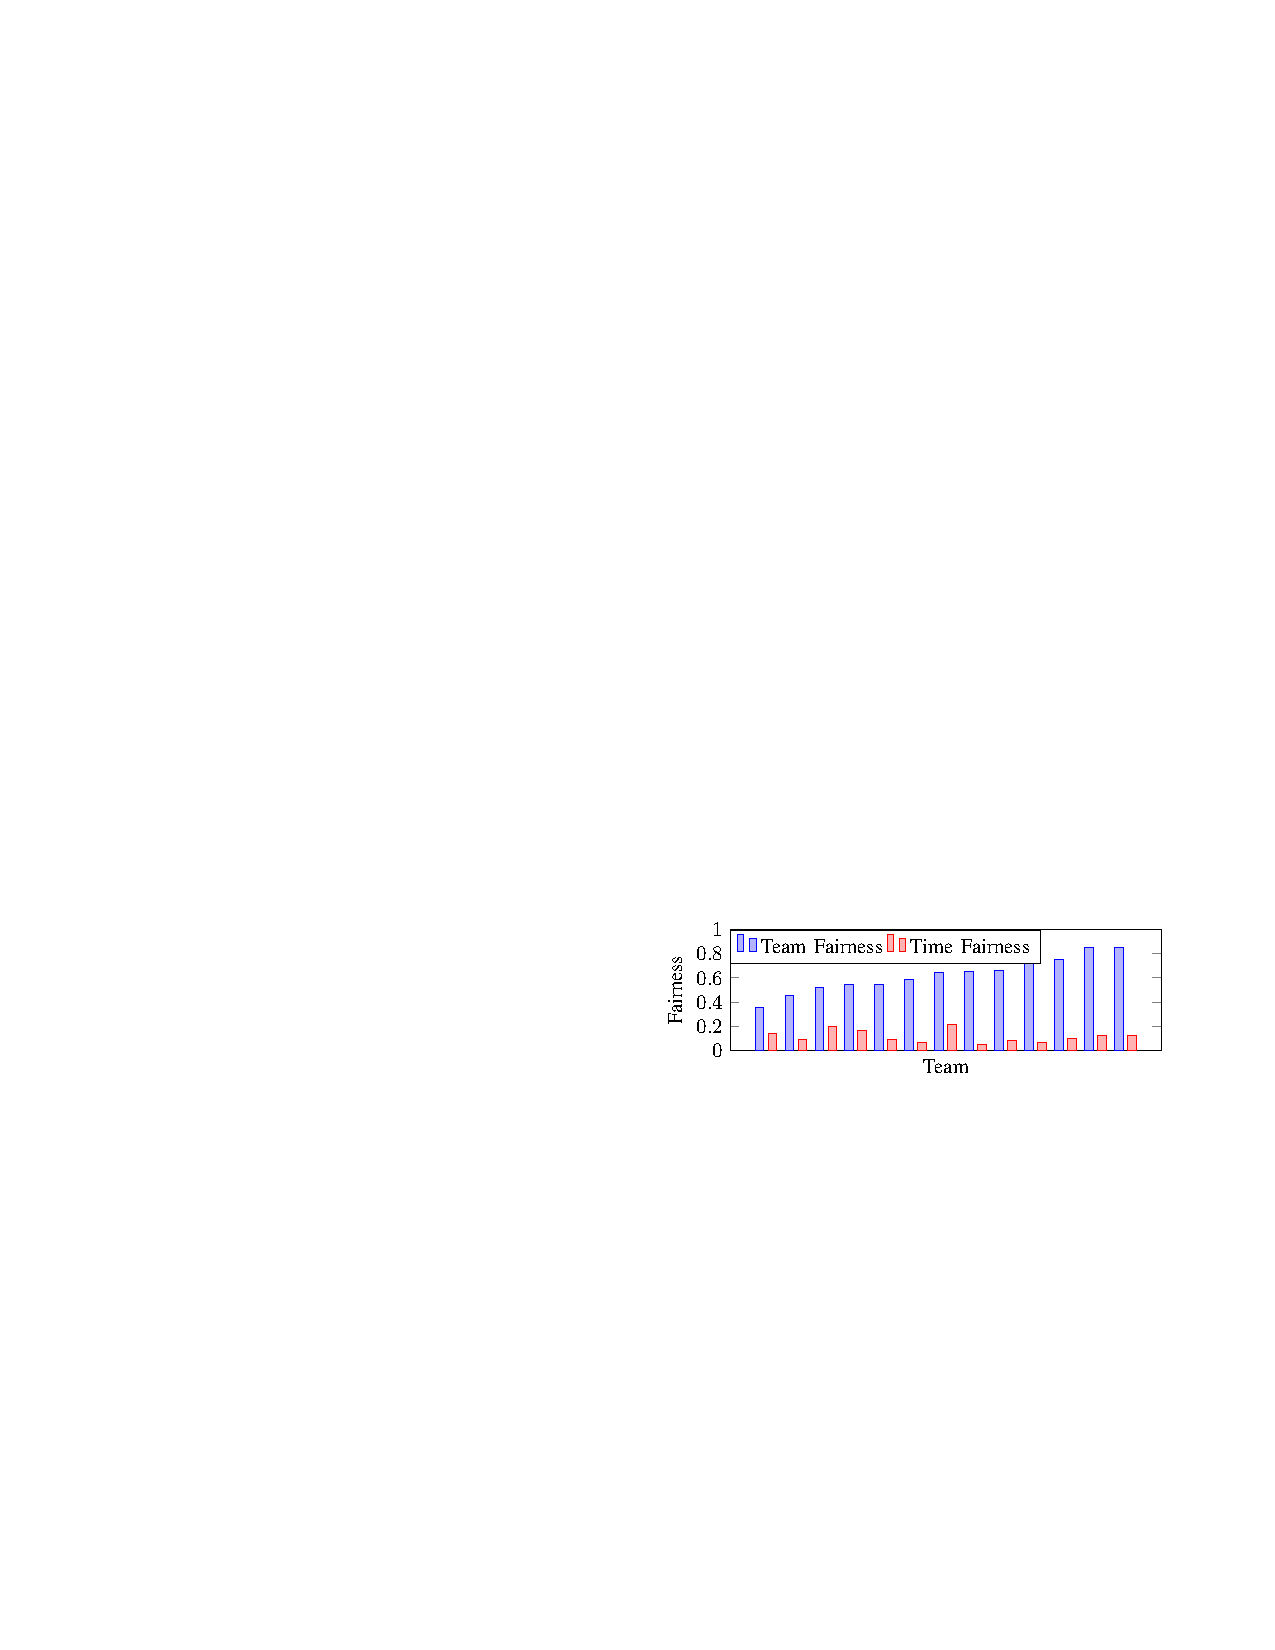
\includegraphics[width=1.0\linewidth]{../figures/FairnessCommits_22_23.pdf}
\caption{Fairness of Commits 2022/23 [n=13; Team Fairness Mean: 0.63, Stddev: 0.15; Time Fairness Mean: 0.12, Stddev: 0.05; Correlation: -0.16]}\label{Fig:Fairness2022/23}
\end{figure}

\begin{figure}[h]
\centering
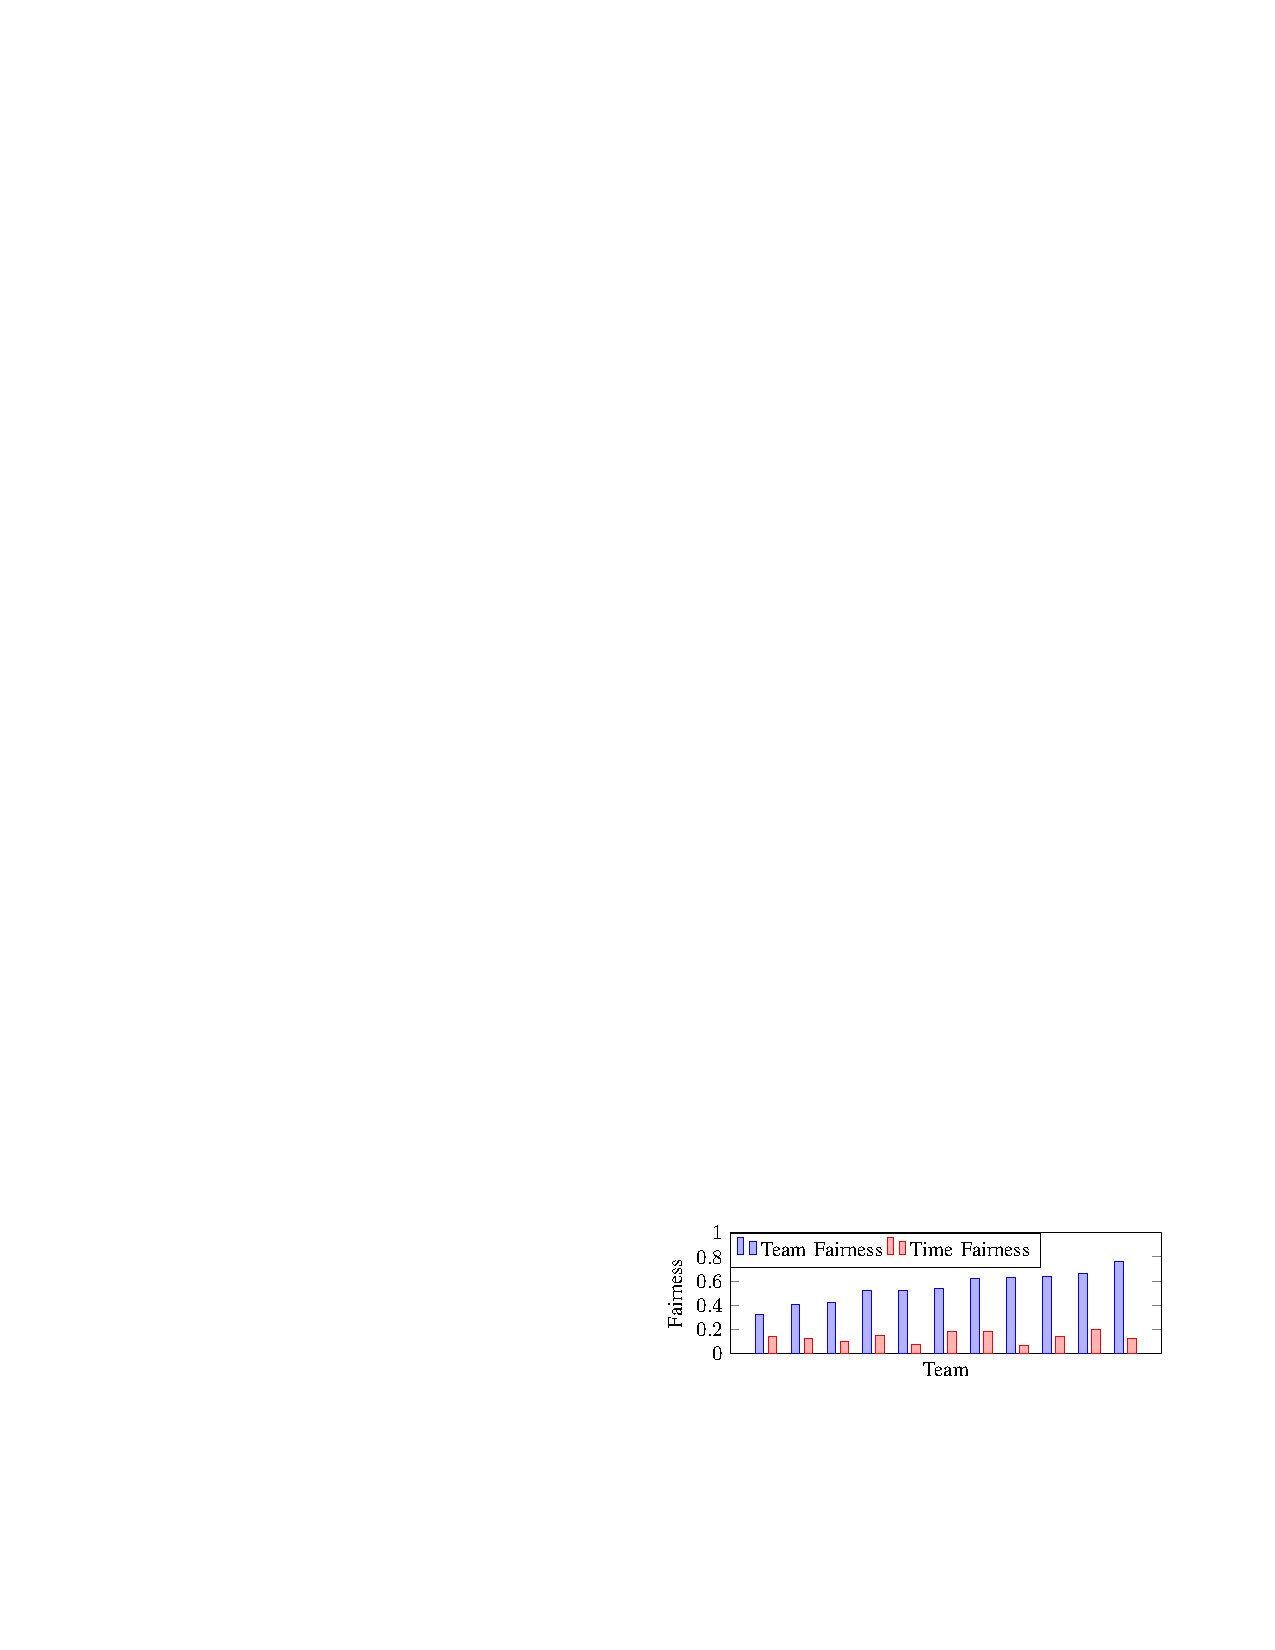
\includegraphics[width=1.0\linewidth]{../figures/FairnessCommits_23_24.pdf}
\caption{Fairness of Commits 2023/24 [n=11; Team Fairness Mean: 0.55, Stddev: 0.13; Time Fairness Mean: 0.14, Stddev: 0.04; Correlation: 0.15]}\label{Fig:Fairness2023/24}
\end{figure}

In the future
\begin{itemize}
    \item Experiment with applying new index to other metrics like lines of
    code, issues created/closed, pull requests created/merged, etc.
    \item Use multiple metrics at once, similar to the multi-Jain fairness
    index 
    \item Investigate correlation between lower fairness values and perceived
    unfairness by the teammates
    \item Investigate whether live access fairness index encourages teams to share
    work or simply encourages them to ``game the system''
\end{itemize}

\section{Conclusions}

\PARstart {P}{reliminary} data suggests that templates, team charters and
productivity monitoring may have an impact.  In the base year we observed 24\%
of commits happening on the due dates, but after partially introducing the
proposed interventions this number improved to 18\%.  Going forward, we propose
an experiment where commit data and interview data is compared between teams
that use the proposed interventions and those that do not.

\begin{figure}[htbp]
  \centering
  
\includegraphics[height=3.2cm,trim={0 0 28.5cm 0},clip]{nserc-logo.jpg}
  \hspace{0.5cm}
  
\includegraphics[height=3.2cm,trim={16.5cm 0 0 0},clip]{ontario@2x-print.png}
  \hspace{0.5cm}
  
\includegraphics[height=3.2cm,trim={0 0.5cm 0 0.48cm},clip]{outreachlogo.png}  
\end{figure}
  
\end{multicols}

\end{document}